\documentclass[12pt,a4paper]{article}{
\usepackage{ctex}
\usepackage{amsmath,amscd,amsbsy,amssymb,latexsym,url,bm,amsthm}
\usepackage{epsfig,graphicx,subfigure}
\usepackage{enumitem,balance}
\usepackage{wrapfig}
\usepackage{mathrsfs,euscript}
\usepackage[usenames]{xcolor}


\usepackage{hyperref}
\usepackage{booktabs}
\usepackage[vlined,ruled,linesnumbered]{algorithm2e}
\hypersetup{colorlinks=true,linkcolor=black}

\newtheorem{theorem}{Theorem}
\newtheorem{problem}{Problem}
\newtheorem{lemma}[theorem]{Lemma}
\newtheorem{proposition}[theorem]{Proposition}
\newtheorem{corollary}[theorem]{Corollary}
\newtheorem{exercise}{Exercise}
\newtheorem*{solution}{Solution}
\newtheorem{definition}{Definition}
\theoremstyle{definition}

\renewcommand{\thefootnote}{\fnsymbol{footnote}}

\newcommand{\postscript}[2]
 {\setlength{\epsfxsize}{#2\hsize}
  \centerline{\epsfbox{#1}}}

\renewcommand{\baselinestretch}{1.0}

\setlength{\oddsidemargin}{-0.365in}
\setlength{\evensidemargin}{-0.365in}
\setlength{\topmargin}{-0.3in}
\setlength{\headheight}{0in}
\setlength{\headsep}{0in}
\setlength{\textheight}{10.1in}
\setlength{\textwidth}{7in}
\makeatletter \renewenvironment{proof}[1][Proof] {\par\pushQED{\qed}\normalfont\topsep6\p@\@plus6\p@\relax\trivlist\item[\hskip\labelsep\bfseries#1\@addpunct{.}]\ignorespaces}{\popQED\endtrivlist\@endpefalse} \makeatother
\makeatletter
\renewenvironment{solution}[1][Solution] {\par\pushQED{\qed}\normalfont\topsep6\p@\@plus6\p@\relax\trivlist\item[\hskip\labelsep\bfseries#1\@addpunct{.}]\ignorespaces}{\popQED\endtrivlist\@endpefalse} \makeatother

\begin{document}
\noindent

%========================================================================
\noindent\framebox[\linewidth]{\shortstack[c]{
\Large{\textbf{Homework 1}}\vspace{1mm}}}
\begin{center}

\footnotesize{ }
\end{center}
\item
\begin{enumerate}
\begin{problem}
Show the Venn-diagram representation for the following sets:
\item [(a)] $(A \cup B) - C$
\item [(b)] $\overline{A \oplus (B \cap C)}$
\begin{solution}
\renewcommand{\qedsymbol}{}
We first assume that any two sets have intersection.\item
then (a) can be as follow:\item
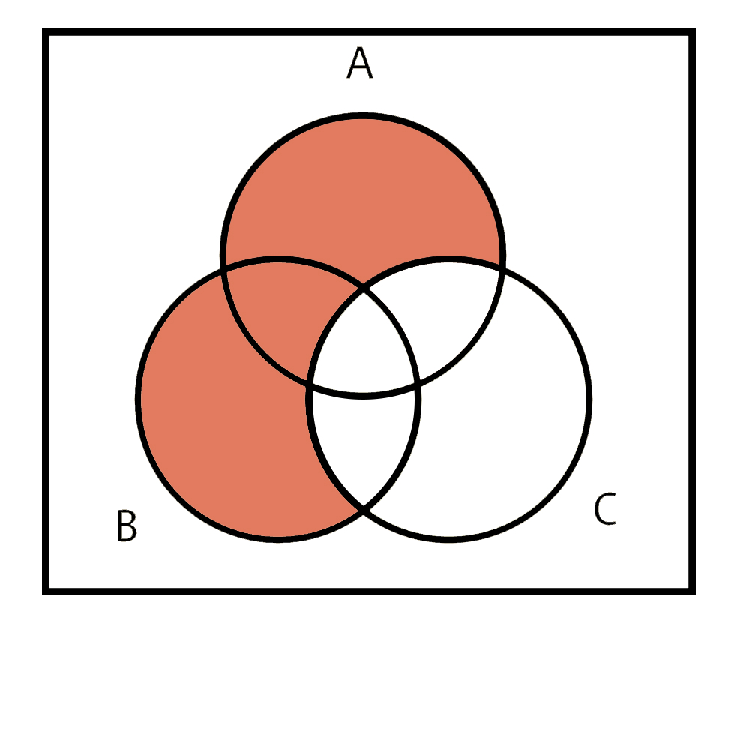
\includegraphics[width=0.4\textwidth]{figures/1_1.pdf}\item
then (a) can be as follow:\item
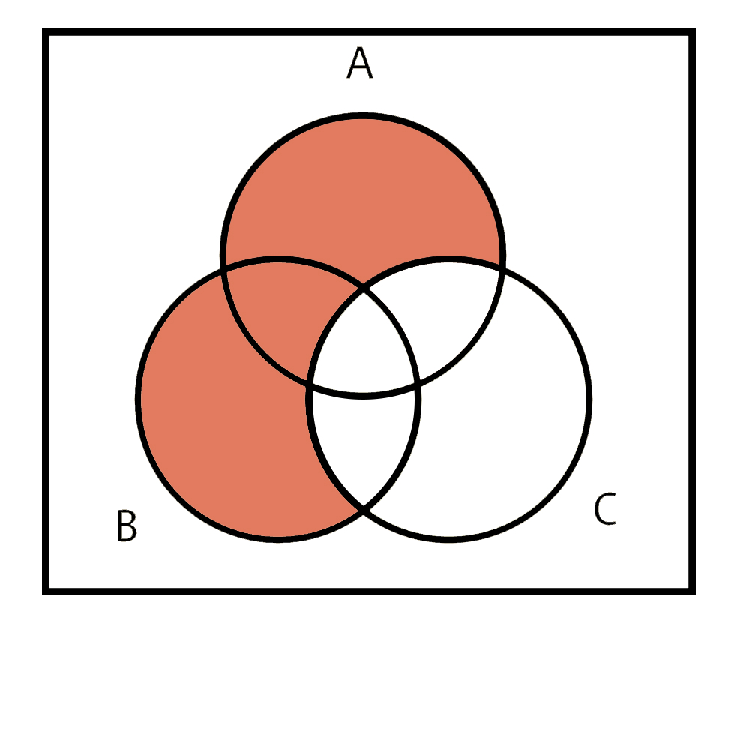
\includegraphics[width=0.4\textwidth]{figures/1_2.pdf}
\end{solution}
\end{problem}
\item
\begin{problem}
For any sets A, B and C, prove that
$$A \cup B = A \cup C, A \cap B = A \cap C\ implies\ B = C.$$
\begin{proof}
\renewcommand{\qedsymbol}{}
We first assume $B \ne C$, so that
$$\exists x \in B ,\ x \notin C$$
$$x \in B \Rightarrow x \in (A \cup B) , A \cup B = A \cup C \Rightarrow x \in (A \cup C)$$
$$since\ x \notin C \Rightarrow x \in A$$
$$since\ x \in A,x \in B \Rightarrow x \in (A \cap B),since\ (A \cap B) = (A \cap C) \Rightarrow x \in (A \cap C)$$
Therefore,$x \in C$it have a contradiction with previous assumption. We can claim $B = C$.
\end{proof}
\end{problem}
\par
\begin{problem}
$\mathcal{}$
1. Show that $\mathcal{R}$ is symmetric iff $\mathcal{R}^{-1} \subset \mathcal{R}$. 
\item
2. Show that $\mathcal{R}$ is transitive iff $\mathcal{R} \circ \mathcal{R} \subset \mathcal{R}$.
\begin{proof}
\renewcommand{\qedsymbol}{}\item
\textbf{1).}\item
necessity: If $\mathcal{R}^{-1} \subset \mathcal{R}$, for any relation $x \rightarrow y \in  \mathcal{R}$, we can claim $y \rightarrow x \in  \mathcal{R}$, therefore $\mathcal{R}$ is $symmetric$.
\item
sufficiency: If $\mathcal{R}$ is $symmetric$, $\mathcal{R}^{-1} = \mathcal{R}$ Therefore $\mathcal{R}^{-1} \subset \mathcal{R}$.
\item
\textbf{2).}\item
necessity: For the definition, $\mathcal{R} \circ \mathcal{R} \subset \mathcal{R}$, $aRb$, $bRc$ $\Rightarrow$ $aRc$. therefore, R is $transitive$.
\item
sufficiency: If R is $transitive$, we can obviously see that combination of two relation $\mathcal{R}$ is satisfied to $\mathcal{R}$. it says that, 
$\mathcal{R} \circ \mathcal{R} \subset \mathcal{R}$.
\end{proof}
\end{problem}
\par
\begin{problem}
Prove that $\mathcal{P}(A) \approx 2^A$, where A is any set and $2^A$ = \{f $\mid$ f : A $\rightarrow$ \{0, 1\} is a function.\}
\begin{proof}
\renewcommand{\qedsymbol}{}
Define a function from $P(A)$ onto $2^A\ as:$\item
For any subset B of A, H(B) is the characteristic function of B:
$$ f_B(x)=\left\{
            \begin{array}{rcl}
            1       &      & {if\ x \in B,}\\
            0     &      &  {if\ x \in A-B.}
            \end{array} \right. $$
H is one-to-one and onto.
\end{proof}
\end{problem}
\par
\begin{problem}
A and B are countable sets. Prove that\item 
1. $A \cup B$ is countable\item
2. $A \times B$ is countable
\begin{proof}\item
\renewcommand{\qedsymbol}{}
\textbf{1).}
We can assume set $A=\{a_1,a_2,a_3,a_4,\cdots \}$, and
$B=\{b_1,b_2,b_3,b_4,\cdots \}$, therefore we can get
$A \cup B =\{a_1,b_1,a_2,b_2,a_3,b_3,a_4,b_4,\cdots \}$\item
We can define a one-to-one mapping from A to $(A \cup B)$, it folows:\item
$$a_1 \Rightarrow a_1$$$$a_2 \Rightarrow b_1$$$$a_3 \Rightarrow a_2$$
$$a_4 \Rightarrow b_2$$$$a_5 \Rightarrow a_3$$$$\cdots$$
Since A is a countable set, We can claim $(A \cup B)$ is countable.\item
\textbf{2).}
Since A is countable, we can first assume $\mid A \mid = k$, $\mid B \mid = p$\item
Then we can define a one-to-one mapping from number set $\mathcal{\omega}$ to $A \times B$.\item
For arithmetic progression $\omega_1=\{c_1,c_2,c_3,\cdots c_p\} = \{2k,4k\cdots 2pk \}$, $\omega_1$ is countable, and $$c_1 \Rightarrow (a_1,b_1)$$
$$c_2 \Rightarrow (a_1,b_2)$$
$$c_3 \Rightarrow (a_1,b_3)$$
$$\dots$$
$$c_i \Rightarrow (a_1,b_i)$$
$$\cdots$$
$$c_p \Rightarrow (a_1,b_p)$$
Then, we can define another countable set, $$\omega_2=\{c_{11},c_{12},c_{13},\cdots c_{1(k-1)},\cdots c_{21},c_{22},c_{23} \cdots c_{2(k-1)}\cdots c_{p1},c_{p2},c_{p3} \cdots c_{p(k-1)}\}$$ and we can define one-to-one mapping:
$$c_{11} \Rightarrow (a_2,b_1)$$$$c_{12} \Rightarrow (a_3,b_1)$$
$$c_{13} \Rightarrow (a_4,b_1)$$$$\cdots$$
$$c_{ij} \Rightarrow (a_{j+1},b_i)$$
Then, we let $\mathcal{\omega}=\omega_1 \cup \omega_2$, for the conclusion in (1), we can claim $\mathcal{\omega}$ is countable.Therefore, $A \times B$ is countable.
\end{proof}
\end{problem}


\end{enumerate}

\vspace{20pt}


%========================================================================
\end{document}
